\chapter{Introduction}
\label{cha:intro}

It is astonishing how, based on the same genetic information coded into the DNA, cells in an organism can differentiate into a variety of specialized types with a multitude of different tasks.
Beginning with a single cell, a temporal, spatial and functional coordination determines the growth and body formation of eukaryotic organisms.
Depending on the cell state, only a fraction of genes is actively transcribed, while others remain repressed.
Acting as an additional regulatory layer, the epigenome describes a set of chemical modifications made to the DNA, controlling, inter alia, the activation and transcription of genes into RNA and ultimately proteins.
Present sequencing technologies and connected bioinformatics provide researchers with the tools to study sequence and epigenetic state down to single cell and single molecule resolution.
Starting 1990 and taking over a decade until completion, the human genome project incorporated an international team of researchers with the aim of deciphering for the first time the genetic blueprint to build a human being. 
Based on elementary sequencing technology, the outcome was already a nearly complete reference sequence including gene annotations.
Since then, the development of high-throughput, next-generation sequencing (NGS) technologies enabled studies of countless organisms, cell types and disease conditions. 
While being very reliable in terms of throughput and accuracy, sequenced fragments of at most few hundreds nucleotides in length still limit the readout from repetitive regions or resolution of long distance dependencies on a single molecule.




\section{Motivation}
\label{sec:intro:motivation}

Most recently, a third-generation of sequencing techniques is introducing new perspectives to the field of genome analysis by generating previously unattainable read lengths with averages in the tens of thousands of nucleotides. 
Still under active development and with frequent improvements, long-read sequencing provides new opportunities by, visually speaking, increasing the size of the puzzle pieces.
Moreover, direct sequencing of DNA and RNA molecules using the nanopore technology facilitates the detection of different types of base modifications.
Modern nanopore sequencing devices, producing large data sets within few days, open therefore a new field of research at the intersection of genomics, computer science and engineering. 
New data types, formats and error characteristics demand here the adaptation of existing and development of new algorithms for bioinformatic software.




\section{Genome Regulation}
\label{sec:intro:bio}

Most cell types of an eukaryotic organism contain a copy of the genetic code in form of folded DNA in the nucleus.
Virtually all mammals have diploid cells with homologous maternal and paternal copies, organized into chromosome pairs with the same genes at the same locations.
While the entire human genome comprises about three billion nucleotides in total, the longest continuous stretch of DNA is the first of 23 chromosome pairs with 247 million base pairs. 
To maintain its integrity and supporting the chromatin structure formation, the DNA is wrapped around octamers of histone proteins called nucleosomes (Fig. \ref{fig:intro:chromatin}).


\begin{figure}[h]
	\centering
	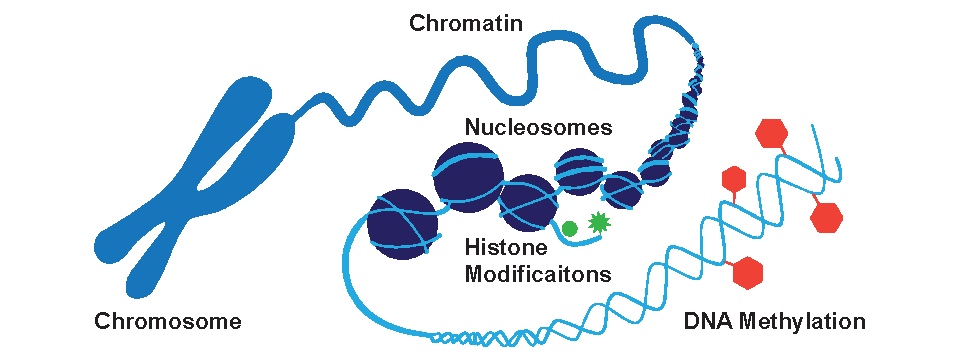
\includegraphics[width=1.0\textwidth]{figures/intro/chromatin.pdf}
	\captionsetup{format=plain}
	\caption[Chromosome to nucleotide structure]{The DNA of each chromosome is wrapped around histones, forming nucleosomes and the chromatin structure. Chemical modifications to histone tails and individual base pairs impact properties and cellular function (Adapted from \cite{zymo2020}).}
	\label{fig:intro:chromatin}
\end{figure}

The \textasciitilde 147bp of DNA directly twisted around each nucleosome is protected against physical access from for instance transcription factors (TFs). 
The dynamic positioning of nucleosomes is therefore part of the epigenetic regulation process during transcription and replication.
Accordingly, nucleosomes are enriched at compacted heterochromatin in mostly inactive genomic regions, while being depleted at regulatory elements such as enhancers, insulators and transcribed genes \cite{Klemm2019}. 
A growing number of chemical modifications to histone tails (H2A, H2B, H3 and H4) is reported to impact inter-nucleosomal interactions, but also leading to recruitment of proteins and complexes involved in transcription, replication and DNA repair \cite{Bannister2011}. 
A well characterized example is the methylation of lysine 79 on the H3 tail (H3K79me3) found at the transcription start sites (TSS) of active genes \cite{Lawrence2016}. 
To be further mentioned in this context are H3K4me3 marking active euchromatin, while H3K9me3 is indicating repressive heterochromatin.
Gene expression may be influenced by nearby active enhancer sites with enrichment of H3K27ac (acetylation).
Finally, repressed and bivalent promoters are modified with H3K27me3 and the combination of H3K4me4 and H3K27me3 respectively.

For embryonic development in mammals, the methylation of cytosine in the CpG-context (5-methylcytosine, 5mC) is a vital epigenetic modification. Prominent examples of its importance are the X-chromosome inactivation in females and genomic imprinting.
Furthermore, DNA methylation is associated with the silencing of transposable elements, shows high levels over actively transcribed gene bodies and correlates with gene repression \cite{Greenberg2019}.
Throughout cellular reprogramming, \textit{de-novo} methylation of the DNA is primarily established by the DNMT3A and DNMT3B enzymes. 
During cell division, the methylation state on the nascent strand in the symmetric CpG-context is restored by the DNMT1 enzyme.
In absence of the maintenance methyltransferase, the 5mC modification is therefore passively lost during each round of replication, but can also be actively removed by oxidation through the TET methylcytosine dioxygenases.
There is a downside of cythosine methylation in the form of potential spontaneous deamination of 5mC, resulting in inherited C to T transitions and ultimately a depletion of CpG sites in mammalian genomes \cite{Holliday1993}. 
The human genome for example, contains only around 29M CpGs instead of 188M as anticipated from the genome size. 
Thus, the conservation under evolutionary pressure underlines the importance of DNA methylation for mammals, while its diverse functions are still not yet fully understood.


On genome wide scale, methylation levels undergo two waves of reprogramming during embryonic development, of which the first one till stem cell state is illustrated in Fig. \ref{fig:intro:methylation}.


\begin{figure}[h]
	\centering
	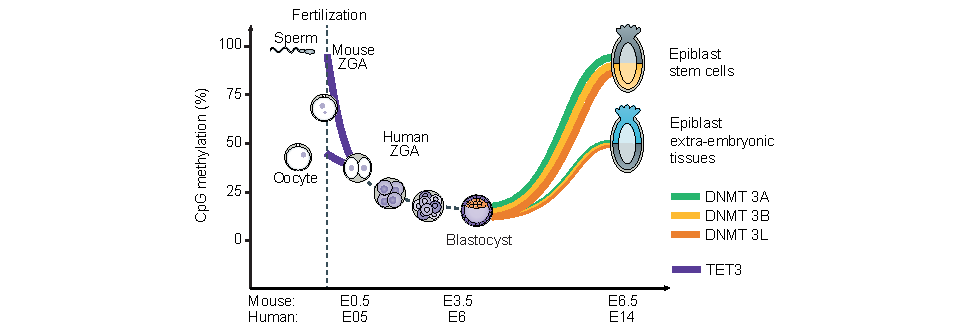
\includegraphics[width=1.0\textwidth]{figures/intro/methylation.pdf}
	\captionsetup{format=plain}
	\caption[DNA methylation reprogramming]{Reprogramming of CpG methylation during embryonic development: Following fertilization and zygotic genome activation (ZGA), mouse and human become actively demethylated by TET3. After blastocyst stage at mouse embryonic day E3.5, DNMT3A and DNMT3B establish \textit{de-novo} methylation under co-expression of DNMT3L. Extra embryonic tissues show a relative hypomethylation compared to the epiblast stem cells (Adapted from \cite{Greenberg2019}).}
	\label{fig:intro:methylation}
\end{figure}

Characteristic for human somatic cells is a genome wide mean methylation of approximately 70\%-80\% \cite{Bird2002}. Averaging the binary 5mC state of individual cells yields mean methylation levels per genomic position. What is striking is the underlying bimodal distribution, with CpG dense regions, also referred to as CpG islands (CGIs), being mostly unmethylated, while the genomic background of more isolated CpGs is mostly methylated \cite{Bird2002}.
A large number of the CGIs in mammals act as promoters, nonetheless the majority remains unmethylated during differentiation and gene silencing is driven by H3K27 methylation \cite{Larsen1992, Greenberg2019}.
A well studied example where DNA methylation is sufficient to repress transcription are imprinted genes, where either the maternal or paternal allele is transcribed, while the other one remains silenced.

Lastly, the DNA-methylation landscape is heavily deregulated in cancer. While sharing a trend towards global hypomethylation and CGI hypermethylation compared to normal tissues (Fig. \ref{fig:intro:cancer}), different tumor types can be identified only based on their methylation footprint \cite{Capper2018}.

\begin{figure}[h]
	\centering
	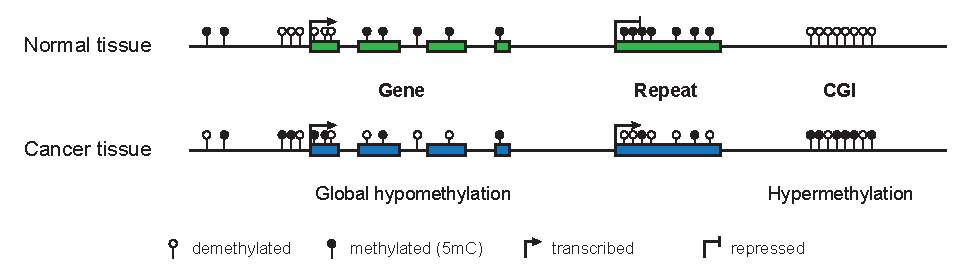
\includegraphics[width=1.0\textwidth]{figures/intro/cancer.pdf}
	\captionsetup{format=plain}
	\caption[DNA methylation in cancer]{Deregulation of DNA methylation patterns in cancer tissues. A global loss across genes and transposable elements (TE) and local gain of methylation levels across CGIs is characteristic for cancer tissue types.}
	\label{fig:intro:cancer}
\end{figure}

While most epigenetic regulators have been discovered and sequencing data for transcriptomes, histone modifications and methylation are available in abundance, the unknown function of high gene body methylation or similarities between extraembryonic tissue and altered methylation in cancer are only two examples of epigenetic regulated processes under active investigation \cite{McGuire2020}.




\section{Sequencing Technologies}
\label{sec:intro:sequencing}

\textit{"For their contributions concerning the determination of base sequences in nucleic acids"}, Walter Gilbert and Frederick Sanger received the 1980 Nobel Prize in Chemistry.
Referred to as first generation or Sanger sequencing, their 'dideoxy method' allowed for the first time to determine the nucleotide sequence of an entire organism with high accuracy \cite{Sanger1977}.
While superseded by second and third generation technologies on genome wide level, Sanger sequencing can still be the method of choice, for instance to verify plasmid sequences, check genotypes or confirm genome editing.

Starting of in 2005 with the 454 Genome Sequencer, the development and commercialization of sequencing by synthesis approaches lead to increasing throughput and broad availability of the second, also termed next generation sequencing (NGS) technologies.
Different platforms, all with typical read lengths of at most few hundred nucleotides include 454, Illumina, SOLiD and Ion torrent.
As marked leader, and with the HiSeq X Ten platform the first company to break the milestone of US\$1000 for a human genome in 2014, Illumina sequencing serves as gold standard and second generation reference in this work \cite{Dijk2014}.

\subsection{Next Generation Sequencing}
\label{subsec:intro:ngs}

Illumina dye sequencing is a high throughput technology, reading millions of short DNA fragments in parallel and with high accuracy (>99.9\%).
As Illustrated in Fig. \ref{fig:intro:sbs}, the process can be divided into library preparation, cluster amplification and the sequencing itself.

Genomic input DNA is first randomly fragmented and ligated to distinct 5' and 3' end adapters.
A polymerase chain reaction (PCR) amplification purifies the library for fragments with sequencing adapters on both ends.
Subsequently, the double stranded DNA is denatured and washed over a flow cell coated with short oligonucleotides, complementary to the sequencing adapters.
The ends of single stranded fragments ligate in sparse density with both, 5' and 3' adapter to the flow cell.
During bridge amplification, the free adapters of single stranded fragments are repeatedly bent to the flow cell surface and the complementary strand is synthesized. 
The denaturation of these double stranded bridges results in a duplication of each template strand into its reverse complement.
Lastly one adapter type is cut away in order to unify the fragment orientation, resulting in dense clusters of identical single stranded DNA fragments.

The actual sequencing process is divided into cycles, each detecting the respective next nucleotide of all clusters in parallel.
During sequencing by synthesis, a polymerase assembles the complementary strand of each fragment from a mix of reversible terminating fluorescent nucleotides.
A blocking group on every nucleotide forces the polymerase to stop after each incorporation, allowing a camera to capture laser-excited fluorescence of all clusters.
Different colors per nucleotide are recognized by the basecalling algorithm and concatenated into a sequence per cluster also referred to as a read.
After unblocking and removal of the fluorophore, the process is repeated until the terminal read length is reached.

Amplification during library preparation and the synthesis during sequencing are virtually error-free.
However, the sequence quality, is affected by clusters running out of phase. 
Sporadic dropouts of the polymerase result in missing nucleotide incorporation within single fragments, leading to an increasing number of fragments lacking behind the cluster's synchronization.
The resulting signal overlap is monitored by the basecaller and translated into a quality score per nucleotide and cluster.
De-phsing of clusters is currently limiting the maximum sequencing length of NGS platforms to \textasciitilde250nt.

\begin{figure}[h]
	\centering
	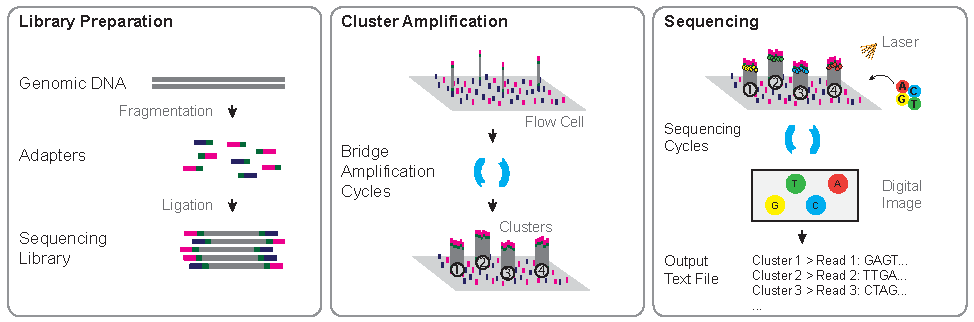
\includegraphics[width=1.0\textwidth]{figures/intro/sbs.pdf}
	\captionsetup{format=plain}
	\caption[Sequencing by synthesis]{Next generation sequencing: The input DNA is fragmented and amplified into clusters of identical reads on a flow cell. Sequencing by synthesis determines the nucleotide sequence of all clusters simultaneously by measuring fluorescence of incorporated bases.}
	\label{fig:intro:sbs}
\end{figure}

Except for de-novo assemblies, a shared first processing step after genome wide sequencing is the alignment.
After fragmentation and sequencing, the genomic origin of each read is initially unknown.
An alignment algorithm determines all possible mappings of a read, commonly allowing for a certain degree of mismatches, insertions and deletions.
Dissimilar read and reference sequence stem from either sequencing errors or differences between reference and the individual genome.
With respect to repetitive elements within mammalian genomes in combination with fragmented sequences, reads may align to multiple genomic positions with the same edit distance.
Depending on the application, a filtering for unique alignments can therefore be necessary.

Enabled by high throughput second generation sequencing, a variety of protocols have been developed in order to extend the application beyond the readout of solely the genomic sequence.
In relation to the already introduced epigenetic regulation, the methods to detect histone modifications and DNA methylation are briefly outlined below.

Chromatin immunoprecipitation sequencing (ChIP-Seq) is a versatile genome-wide method to identify binding sites of DNA-associated proteins.
Crosslinking of DNA-protein complexes fixes the current position of for instance histones. 
A fragmentation step separates the DNA in protein-bound and unbound sections.
A modification specific magnetic antibody is used, to immunoprecipitate the complex and pull down only sequence fragments directly adjacent to a histone carrying the epigenetic modification of interest.
Sequencing and data analysis reveal histone modifications as peaks from local accumulations of reads.

Whole genome bisulfite sequencing (WGBS) is the state of the art method to detect methylation on individual molecules \cite{Frommer1992}.
A reaction with sodium bisulfite converts any unmethylated cytosine to uracil, while 5-methylcytosine remains unchanged and consequently encodes the methylation state into the sequence. 
Uracil and thymine are both amplified and sequenced as thymine (T), while only methylated cytosine is read as C.
At genomic CG positions, a read alignment containing a CG indicates therefore a previously methylated site, a mismatching TG indicates an unmethylated site.
The methylation state of individual reads is then summarized to a methylation rate per genomic position.
A minimum coverage of 5X to 10X has been shown to be robust against inter-cell variability and allow the comparison across samples \cite{Ziller2015}.




\subsection{Third Generation Sequencing}
\label{subsec:intro:tgs}

In contrast to high-throughput short-read sequencing, third generation long-read technologies do not necessarily require amplification and yield read lengths in the range of tens of thousands nucleotides. 
Single-molecule real-time sequencing (SMRT), introduced by Pacific Biosciences (PacBio) in 2011, is considered to be the first commercially available long-read technology \cite{Dijk2018}.
While the idea of nanopore sequencing goes back to the 1980s, it took until 2014 to release the pocket sized MinION as first device by Oxford Nanopore Technologies (ONT) \cite{Deamer2016}.

Single-molecule real-time sequencing is based on individual DNA fragments fixed into zero-mode waveguides (ZMW).
For the library preparation, genomic input DNA is fragmented to typically 8-15kB and ligated to hairpin adapters.
Termed SMRTbell, each molecule is denatured and as circular single stranded DNA fixed into the ZMWs on the flow cell.
During the sequencing process, a polymerase located at the transparent bottom of each well synthesizes the complementary strand from nucleotides labeled with fluorescent dye.
At a speed of 10nt/s, light impulses from laser-excited fluorescence are the primary measurement to determine the nucleotide sequence of each read (Fig. \ref{fig:intro:longread}, left box).
According to the manufacturer, a Sequel IIe flow cell with 8M ZMWs can generate up to 4M reads during 30h of sequencing. \footnote{https://www.pacb.com/products-and-services/sequel-system, accessed 12/2020}
More recently, PacBio advanced to high-fidelity (HiFi) reads, which are generated as consensus sequence from multiple passes of the polymerase around the template strand.
HiFi reads increase the single read accuracy to >99\% at the cost of the overall read length.
Without PCR amplification of the input material, epigenetic base modifications remain on the sample DNA and impact the output signal as extended pauses between light impulses.
The most prominent example is the detection of bacterial 6-methyladenine (6mA). 
However, the sensitivity to 5mC remains a proof of concept and studies reporting its successful application could not be identified.

\begin{figure}[h]
	\centering
	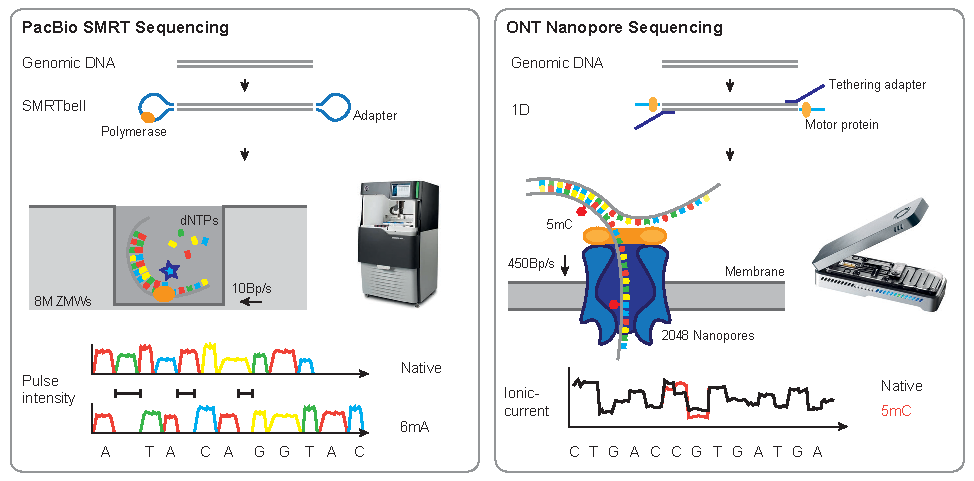
\includegraphics[width=1.0\textwidth]{figures/intro/long_read.pdf}
	\captionsetup{format=plain}
	\caption[Long read sequencing]{PacBio SMRT and ONT nanopore sequencing: Single-molecule real-time sequencing by circular synthesis of secondary strands measured as laser-excited fluorescence pulses. Nanopore sequencing of DNA and RNA strands measured as changes in ionic currents while traversing through the pore. Base modifications can be directly detected as either extended pulse pauses or characteristic current level differences.}
	\label{fig:intro:longread}
\end{figure}

Interestingly, both NGS and SMRT sequencing technologies utilize the fluorescence signal of nucleotides synthesized into a complementary strand of the sequenced DNA fragment.
Nanopore sequencing follows a fundamentally different principle.
The sequencing is no longer based on the synthesis of a second strand, as individual pores asynchronously read multiple molecules one after the other, in contrast to the previous parallel approaches.
Additionally, nanopore sequencing can not only process double stranded DNA, but also directly read single stranded RNA.
The nanopore flow cell is build of pores embedded into a membrane separating two wells.
After loading the flow cell with a run buffer, a voltage applied over the membrane causes a constant ionic current through each pore.
While always in the range of pico ampere, any molecule passing through the pore reduces the level of the ionic current depending on its physical and chemical properties.

Initial steps of the library preparation like fragmentation, end-repair and size selection are shared across long read technologies.
For nanopore sequencing, a motor protein and a tethering adapter are ligated to both ends of the input DNA.
The tethering adapter helps guiding the reads to pores on the flow-cell, where the motor protein is attaching to the pore and controlling the sequencing speed to \textasciitilde450nt/s for DNA or \textasciitilde70nt/s for RNA.
During the sequencing process, the double strand is split in front of the pore and only one strand is read.
The ionic current per pore serves as a proxy signal for the molecule passing through, is recorded and finally translated into a nucleotide sequence by the basecalling algorithm (Fig. \ref{fig:intro:longread}, right box).
Without amplification of the input, the nanopore is sensitive to different base modifications including 5-methylcytosine, 6-methyladenine and even synthetic base analogues.

Among other devices distributed by Oxford Nanopore Technologies, the MinION in particular is gaining prominence. 
The portability and very low acquisition costs open new perspectives of real time sequencing in the field or in clinical settings.
Operational directly in the lab and sensitive to base modifications relevant in mouse and human, the nanopore platform is deemed to be the preferable third generation technology for an epigenetics lab.




\section{Structure}
\label{sec:intro:structure}

The submitted work is structured into four major parts, moving from a zoomed out view into the literature over the development of a universal nanopore data processing pipeline into the signal processing and application development for human genetics.

\textbf{Chapter \ref{cha:state_of_art} - State of the Art} %\\[0.2em]

Entitled as \textit{the third revolution in sequencing technology}, Van Dijk et al. \cite{Dijk2018} outline the potentials within an innovative and rapidly developing field of research using third generation sequencing.
It is indispensable to keep track of latest developments in the nanopore field, highlighted for instance by the single read accuracy improvements from 87\% to 95\% modal, solely by enhanced basecalling algorithms applicable to existing data.
This chapter aims to provide a comprehensive overview of use cases for nanopore sequencing, backed by the computational analysis of millions of publications forming a literature graph of keywords and citations.
Based on in-house data, throughput and accuracy summaries for sequence and methylation detection complete the assessment of the current status of the technology.


\textbf{Chapter \ref{cha:nanopype} - Nanopype}

The widespread availability of the nanopore sequencing platform is sparking the development of novel bioinformatic software.
Nonetheless, the streamlined raw data handling and processing of more complex workflows was lacking consistent pipelines, impeding the reproducibility across projects and labs.
This chapter covers the development of the modular Snakemake pipeline \textit{Nanopype}.
As a set of nanopore specific workflows, it covers the most common use cases such as basecalling, alignment, methylation and structural variant detection.
Deployed as python module with automatically build and tested software containers, the pipeline maintains all of it's internal dependencies including the version control of integrated tools.
\textit{Nanopype} is the baseline for subsequent projects and facilitates the rapid development of own and integration of third party software.


\textbf{Chapter \ref{cha:signal} - Signal Processing}

The interplay of a protein nanopore and molecules passing through it causes a characteristic ionic current signal.
In the past, advancing algorithms led to improved single read accuracy, detection of epigenetic base modifications and efficient barcode de-multiplexing based on raw nanopore reads.
For the development of novel applications, the raw signal may be the input of choice, allowing to bypass basecaller induced errors.
This chapter covers basic raw signal processing methods including simulation, normalization and signal alignment.
A flexible raw signal framework enables the seamless integration of signal and sequence space information.
 

\textbf{Chapter \ref{cha:strique} - STRique}

Sequencing of genomic regions previously inaccessible for short read technologies is a key advantage of long reads.
Stretches of repetitive DNA with low sequence complexity are difficult to investigate once they become longer than the read length.
Short tandem repeats (STR) are an example of repeat elements being expanded to multiple thousand nucleotides in length in disease cases.
Enabled by our processing framework and signal analysis methods, \textit{STRique} facilitates the precise analysis of STRs in synthetic and patient samples.
Our method allows for the first time to exactly quantify the length of STRs and integrate repeat count and methylation state on single molecule level.


This thesis concludes with a summary and discussion of the results.
An outlook includes the assessment, where third generation sequencing technologies in general and nanopore sequencing in particular are presumably replacing short reads, where they are appropriate to supplement and where short reads are likely to stay state of the art.
Taken together, this work aims to provide the reader with an overview of the nanopore field in general, propose streamlined processing and novel signal analysis methods and contrast opportunities against challenges within a technology driven research branch.







